%%%%%%%%%%%%%%%%%%%%% chapter.tex %%%%%%%%%%%%%%%%%%%%%%%%%%%%%%%%%
%
% sample chapter
%
% Use this file as a template for your own input.
%
%%%%%%%%%%%%%%%%%%%%%%%% Springer-Verlag %%%%%%%%%%%%%%%%%%%%%%%%%%
%\motto{Use the template \emph{chapter.tex} to style the various elements of your chapter content.}

\chapter{Rosetta Code Tasks starting with A}
\label{rosettacode-numbers}

\section*{A+B}

\textbf{A+B} - in programming contests, classic problem, which is given
so contestants can gain familiarity with online judging system being
used.

\textbf{Problem statement:} Given 2 integer numbers, A and B. One
needs to find their sum.

\textbf{Input data:} Two integer numbers are written in the input
stream, separated by space.

\begin{figure}[H]
\centering
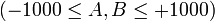
\includegraphics[scale=.6]{graphics/a344abb2a9a00cb2de6679a485115ce3.png}
% \caption{(-1000 \textbackslash{}le A,B \textbackslash{}le +1000)}
\end{figure}

\textbf{Output data:} The required output is one integer: the sum of A
and B.

\textbf{Example:}

\ctable[pos = H, center, botcap]{lc}{% notes
}{% rows
\FL
 Input & Output 
\ML
\texttt{2 2} & \texttt{4} 
\NN
\texttt{3 2} & \texttt{5} 
\LL
}

% \noalign{\medskip}


\begin{wideverbatim}

(+ (read) (read))
3 4
-> 7

\end{wideverbatim}

\pagebreak{}
\section*{Abstract type}

\textbf{Abstract type} is a type without instances or without
definition.

For example in object-oriented programming using some languages,
abstract types can be partial implementations of other types, which
are to be derived there-from. An abstract type may provide
implementation of some operations and/or components. Abstract types
without any implementation are called \textbf{interfaces}. In the
languages that do not support multiple inheritance (Ada, Java),
classes can, nonetheless, inherit from multiple interfaces. The
languages with multiple inheritance (like C++) usually make no
distinction between partially implementable abstract types and
interfaces. Because the abstract type's implementation is incomplete,
OO languages normally prevent instantiation from them (instantiation
must derived from one of their descendant classes).

The term \textbf{abstract datatype} also may denote a type, with an
implementation provided by the programmer rather than directly by the
language (a \textbf{built-in} or an inferred type). Here the word
\emph{abstract} means that the implementation is abstracted away,
irrelevant for the user of the type. Such implementation can and
should be hidden if the language supports separation of implementation
and specification. This hides complexity while allowing the
implementation to change without repercussions on the usage. The
corresponding software design practice is said to follow the
information hiding principle.

It is important not to confuse this \emph{abstractness} (of
implementation) with one of the \textbf{abstract type}. The latter is
abstract in the sense that the set of its values is empty. In the sense
of implementation abstracted away, all user-defined types are abstract.

In some languages, like for example in Objective Caml which is strongly
statically typed, it is also possible to have \textbf{abstract types}
that are not OO related and are not an abstractness too. These are
\emph{pure abstract types} without any definition even in the
implementation and can be used for example for the type algebra, or for
some consistence of the type inference. For example in this area, an
abstract type can be used as a phantom type to augment another type as
its parameter.

\textbf{Task}: show how an abstract type can be declared in the
language. If the language makes a distinction between interfaces and
partially implemented types illustrate both.


\begin{wideverbatim}

# In PicoLisp there is no formal difference between abstract and concrete
# classes, just a naming convention where abstract classes start with a
# lower case character after the '+' (the naming convention for classes).
# This tells the programmer that this class has not sufficient methods
# defined to survive on its own.

(class +abstractClass)

(dm someMethod> ()
   (foo)
   (bar) )

\end{wideverbatim}

\pagebreak{}
\section*{Accumulator factory}


A problem posed by Paul Graham is that of creating a function that
takes a single (numeric) argument and which returns another function
that is an accumulator. The returned accumulator function in turn also
takes a single numeric argument, and returns the sum of all the
numeric values passed in so far to that accumulator (including the
initial value passed when the accumulator was created).

The detailed rules are at
\href{http://paulgraham.com/accgensub.html}{http://paulgraham.com/accgensub.html}
and are reproduced here for simplicity (with additions in \emph{small
  italic text}).

Before you submit an example, make sure the function

\begin{enumerate}
\item
  Takes a number n and returns a function (lets call it g), that takes a
  number i, and returns n incremented by the accumulation of i from
  every call of function g(i).\\Although these exact function and
  parameter names need not be used
\item
  Works for any numeric type-- i.e. can take both ints and floats and
  returns functions that can take both ints and floats. (It is not
  enough simply to convert all input to floats. An accumulator that has
  only seen integers must return integers.) \emph{(i.e., if the language
  doesn't allow for numeric polymorphism, you have to use overloading or
  something like that)}
\item
  Generates functions that return the sum of every number ever passed to
  them, not just the most recent. \emph{(This requires a piece of state
  to hold the accumulated value, which in turn means that pure
  functional languages can't be used for this task.)}
\item
  Returns a real function, meaning something that you can use wherever
  you could use a function you had defined in the ordinary way in the
  text of your program. \emph{(Follow your language's conventions
  here.)}
\item
  Doesn't store the accumulated value or the returned functions in a way
  that could cause them to be inadvertently modified by other code.
  \emph{(No global variables or other such things.)}
\end{enumerate}

E.g. if after the example, you added the following code (in a made-up
language) \emph{where the factory function is called foo}:

\begin{verbatim}
x = foo(1); x(5); foo(3);print x(2.3);
\end{verbatim}

It should print \texttt{8.3}. \emph{(There is no need to print the form
of the accumulator function returned by \texttt{foo(3)}; it's not part
of the task at all.)}

The purpose of this task is to create a function that implements the
described rules. It need not handle any special error cases not
described above. The simplest way to implement the task as described
is typically to use a closure, providing the language supports them.

Where it is not possible to hold exactly to the constraints above,
describe the deviations.


\begin{wideverbatim}

(de accumulator (Sum)
   (curry (Sum) (N)
      (inc 'Sum N) ) )

(def 'a (accumulator 7))
(a 1)  # Output: -> 8
(a 2)  # Output: -> 10
(a -5)  # Output: -> 5

\end{wideverbatim}

\pagebreak{}
\section*{Ackermann function}

The
\textbf{\href{http://en.wikipedia.org/wiki/Ackermann\_function}{Ackermann
function}} is a classic recursive example in computer science. It is a
function that grows very quickly (in its value and in the size of its
call tree). It is defined as follows:

\begin{figure}[H]
\centering
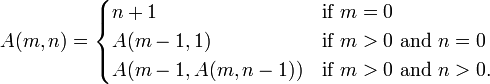
\includegraphics[scale=.6]{graphics/0ae4053de098cc9554752b190a38bc56.png}
% \caption{ A(m, n) = \textbackslash{}begin\{cases\} n+1 \&
% \textbackslash{}mbox\{if \} m = 0 \textbackslash{}\textbackslash{}
% A(m-1, 1) \& \textbackslash{}mbox\{if \} m \textgreater{} 0
% \textbackslash{}mbox\{ and \} n = 0 \textbackslash{}\textbackslash{}
% A(m-1, A(m, n-1)) \& \textbackslash{}mbox\{if \} m \textgreater{} 0
% \textbackslash{}mbox\{ and \} n \textgreater{} 0.
% \textbackslash{}end\{cases\} }
\end{figure}

Its arguments are never negative and it always terminates. Write a
function which returns the value of \emph{A}(\emph{m},\emph{n}).
Arbitrary precision is preferred (since the function grows so quickly),
but not required.

\begin{wideverbatim}

(de ack (X Y)
   (cond
      ((=0 X) (inc Y))
      ((=0 Y) (ack (dec X) 1))
      (T (ack (dec X) (ack X (dec Y)))) ) )

\end{wideverbatim}

\pagebreak{}
\section*{Active Directory/Connect}

The task is to establish a connection to an Active Directory or
Lightweight Directory Access Protocol server.

\begin{wideverbatim}

(unless (=0 (setq Ldap (native "libldap.so" "ldap_open" 'N "example.com" 389)))
   (quit "Can't open LDAP") )

(native "libldap.so" "ldap_simple_bind_s" 'I Ldap "user" "password")

\end{wideverbatim}

\pagebreak{}
\section*{Active Directory/Search for a user}

Make sure you Connect to Active Directory

\begin{wideverbatim}

(de ldapsearch (Sn)
   (in
      (list "ldapsearch" "-xH" "ldap://db.debian.org"
         "-b" "dc=debian,dc=org"
         (pack "sn=" Sn) )
      (list
         (cons 'cn (prog (from "cn: ") (line T)))
         (cons 'uid (prog (from "uid: ") (line T))) ) ) )

Test:

: (ldapsearch "Fischer")
-> ((cn . "Mika") (uid . "mf"))

\end{wideverbatim}

\pagebreak{}
\section*{Active object}

In object-oriented programming an object is active when its state
depends on clock. Usually an active object encapsulates a task that
updates the object's state. To the outer world the object looks like a
normal object with methods that can be called from outside.
Implementation of such methods must have a certain synchronization
mechanism with the encapsulated task in order to prevent object's
state corruption.

A typical instance of an active object is an animation widget. The
widget state changes with the time, while as an object it has all
properties of a normal widget.

% Animation is the foundation of a great many parts of graphical user
% interfaces, including both the fancy effects when things change used in
% window managers, and of course games. The core of any animation system
% is a scheme for periodically changing the display while still remaining
% responsive to the user. This task demonstrates this.

% Create a window containing the string "\texttt{Hello World! }" (the
% trailing space is significant). Make the text appear to be rotating
% right by periodically removing one letter from the end of the string and
% attaching it to the front. When the user clicks on the text, it should
% reverse its direction.

\textbf{The task}

Implement an active integrator object. The object has an input and
output. The input can be set using the method \emph{Input}. The input is
a function of time. The output can be queried using the method
\emph{Output}. The object integrates its input over the time and the
result becomes the object's output. So if the input is
\emph{K}(\emph{t}) and the output is \emph{S}, the object state \emph{S}
is changed to \emph{S} + (\emph{K}(\emph{t}\textsubscript{1}) +
\emph{K}(\emph{t}\textsubscript{0})) * (\emph{t}\textsubscript{1} -
\emph{t}\textsubscript{0}) / 2, i.e. it integrates \emph{K} using the
trapeze method. Initially \emph{K} is constant 0 and \emph{S} is 0.

In order to test the object:

\begin{enumerate}
\item
  set its input to sin (2$\pi$ \emph{f t}), where the frequency
  \emph{f}=0.5Hz. The phase is irrelevant.
\item
  wait 2s
\item
  set the input to constant 0
\item
  wait 0.5s
\end{enumerate}

Verify that now the object's output is approximately 0 (the sine has
the period of 2s). The accuracy of the result will depend on the OS
scheduler time slicing and the accuracy of the clock.



\begin{wideverbatim}

(load "@lib/math.l")

(class +Active)
# inp val sum usec

(dm T ()
   (unless (assoc -100 *Run)           # Install timer task
      (task -100 100                   # Update objects every 0.1 sec
         (mapc 'update> *Actives) ) )
   (=: inp '((U) 0))                   # Set zero input function
   (=: val 0)                          # Initialize last value
   (=: sum 0)                          # Initialize sum
   (=: usec (usec))                    # and time
   (push '*Actives This) )             # Install in notification list

(dm input> (Fun)
   (=: inp Fun) )

(dm update> ()
   (let (U (usec)  V ((: inp) U))      # Get current time, calculate value
      (inc (:: sum)
         (*/
            (+ V (: val))              # (K(t[1]) + K(t[0])) *
            (- U (: usec))             # (t[1] - t[0]) /
            2.0 ) )                    # 2.0
      (=: val V)
      (=: usec U) ) )

(dm output> ()
   (format (: sum) *Scl) )             # Get result

(dm stop> ()
   (unless (del This '*Actives)        # Removing the last active object?
      (task -100) ) )                  # Yes: Uninstall timer task

(de integrate ()                       # Test it
   (let Obj (new '(+Active))           # Create an active object
      (input> Obj                      # Set input function
         '((U) (sin (*/ pi U 1.0))) )  # to sin(π * t)
      (wait 2000)                      # Wait 2 sec
      (input> Obj '((U) 0))            # Reset input function
      (wait 500)                       # Wait 0.5 sec
      (prinl "Output: " (output> Obj)) # Print return value
      (stop> Obj) ) )                  # Stop active object

\end{wideverbatim}

\pagebreak{}
\section*{Add a variable to a class instance at runtime}

Demonstrate how to dynamically add variables to an object (a class
instance) at runtime.

This is useful when the methods/variables of an instance are based on
a data file that isn't available until runtime. Hal Fulton gives an
example of creating an OO CSV parser at
\href{http://www.devsource.com/article2/0,1759,1928562,00.asp}{An
  Exercise in Metaprogramming with Ruby}. This is referred to as
``monkeypatching'' by Pythonistas and some others.


\begin{wideverbatim}

In general, all instance variables in PicoLisp are dynamically created at
runtime.

: (setq MyObject (new '(+MyClass)))       # Create some object
-> \$385605941
: (put MyObject 'newvar '(some value))    # Set variable
-> (some value)
: (show MyObject)                         # Show the object
\$385605941 (+MyClass)
   newvar (some value)
-> \$385605941

\end{wideverbatim}

\pagebreak{}
\section*{Address of a variable}

\textbf{Basic Data Operation:} This is a basic data operation. It
represents a fundamental action on a basic data type.

You may see other such operations in the Basic Data Operations
category, or:

\textbf{Integer Operations:} Arithmetic \textbar{} Comparison

\textbf{Boolean Operations:} Bitwise \textbar{} Logical

\textbf{String Operations:} Concatenation \textbar{} Interpolation
\textbar{} Matching

\textbf{Memory Operations:} Pointers \& references \textbar{} \textbf{Addresses}

Demonstrate how to get the address of a variable and how to set the
address of a variable.


\begin{wideverbatim}

The PicoLisp function '[http://software-lab.de/doc/refA.html#adr adr]' returns
the address of a variable. A variable may be either a symbol or a cons pair in
PicoLisp.

The returned address is a number representing an encoded pointer. For symbols,
it is a negative number, and for cons pairs a positive number. The same function
'adr' can then be used to convert that pointer back to the original object.

: (setq X 7)
-> 7

: (adr 'X)
-> -2985527269106

: (val (adr -2985527269106))
-> 7

: (set (adr -2985527269106) '(a b c))
-> (a b c)

: X
-> (a b c)

\end{wideverbatim}

\pagebreak{}
\section*{Align columns}

Given a text file of many lines, where fields within a line are
delineated by a single `dollar' character, write a program that aligns
each column of fields by ensuring that words in each column are
separated by at least one space. Further, allow for each word in a
column to be either left justified, right justified, or center
justified within its column.

Use the following text to test your programs:

\begin{wideverbatim}
Given$a$text$file$of$many$lines,$where$fields$within$a$line$
are$delineated$by$a$single$'dollar'$character,$write$a$program
that$aligns$each$column$of$fields$by$ensuring$that$words$in$each$
column$are$separated$by$at$least$one$space.
Further,$allow$for$each$word$in$a$column$to$be$either$left$
justified,$right$justified,$or$center$justified$within$its$column.
\end{wideverbatim}

Note that:

\begin{enumerate}
\item
  The example input texts lines may, or may not, have trailing dollar
  characters.
\item
  All columns should share the same alignment.
\item
  Consecutive space characters produced adjacent to the end of lines are
  insignificant for the purposes of the task.
\item
  Output text will be viewed in a mono-spaced font on a plain text
  editor or basic terminal.
\item
  The minimum space between columns should be computed from the text and
  not hard-coded.
\item
  It is \emph{not} a requirement to add separating characters between or
  around columns.
\end{enumerate}



\begin{wideverbatim}

(let Sizes NIL                         # Build a list of sizes
   (let Lines                          # and of lines
      (make
         (in "input.txt"                     # Reading input file
            (while (split (line) "$")        # delimited by '$'
               (let (L (link (mapcar pack @))  S Sizes)
                  (setq Sizes                   # Maintain sizes
                     (make
                        (while (or L S)
                           (link
                              (max
                                 (inc (length (pop 'L)))
                                 (pop 'S) ) ) ) ) ) ) ) ) )
      (for L Lines                                 # Print lines
         (prinl (apply align L (mapcar - Sizes))) )   # left aligned
      (prinl)
      (for L Lines
         (prinl (apply align L Sizes)) )              # right aligned
      (prinl)
      (for L Lines
         (prinl (apply center L Sizes)) ) ) )         # and centered

\end{wideverbatim}

\pagebreak{}
\section*{Amb}

Define and give an example of the \emph{\textbf{Amb}} operator.

The Amb operator takes some number of expressions (or values if that's
simpler in the language) and nondeterministically yields the one or
fails if given no parameter, amb returns the value that doesn't lead to
failure.

The example is using amb to choose four words from the following
strings:

set 1: ``the'' ``that'' ``a''

set 2: ``frog'' ``elephant'' ``thing''

set 3: ``walked'' ``treaded'' ``grows''

set 4: ``slowly'' ``quickly''

It is a failure if the last character of word 1 is not equal to the
first character of word 2, and similarly with word 2 and word 3, as well
as word 3 and word 4. (the only successful sentence is ``that thing
grows slowly'').


\begin{wideverbatim}

For backtracking, Pilog (PicoLisp Prolog) is the natural choice.

(be amb (@E @Lst)
   (lst @E @Lst) )

(be joins (@Left @Right)
   (@T last (chop (-> @Left)))
   (@R car (chop (-> @Right)))
   (or
      ((equal @T @R))
      ((amb @ NIL)) ) )  # Explicitly using amb fail as required

(be ambExample ((@Word1 @Word2 @Word3 @Word4))
  (amb @Word1 ("the" "that" "a"))
  (amb @Word2 ("frog" "elephant" "thing"))
  (amb @Word3 ("walked" "treaded" "grows"))
  (amb @Word4 ("slowly" "quickly"))
  (joins @Word1 @Word2)
  (joins @Word2 @Word3)
  (joins @Word3 @Word4) )

Output:

: (? (ambExample @Result))
 @Result=("that" "thing" "grows" "slowly")
-> NIL

\end{wideverbatim}

\pagebreak{}
\section*{Anagrams}

Two or more words can be composed of the same characters, but in a
different order. Using the word list at
\href{http://www.puzzlers.org/pub/wordlists/unixdict.txt}{http://www.puzzlers.org/pub/wordlists/unixdict.txt},
find the sets of words that share the same characters that contain the
most words in them.


\begin{wideverbatim}

A straight-forward implementation using 'group' takes 48 seconds
on a 1.7 GHz Pentium:

(flip
   (by length sort
      (by '((L) (sort (copy L))) group
         (in "unixdict.txt" (make (while (line) (link @)))) ) ) )

Using a binary tree with the 'idx' function, it takes only 0.42 seconds
on the same machine, a factor of 100 faster:

(let Words NIL
   (in "unixdict.txt"
      (while (line)
         (let (Word (pack @)  Key (pack (sort @)))
            (if (idx 'Words Key T)
               (push (car @) Word)
               (set Key (list Word)) ) ) ) )
   (flip (by length sort (mapcar val (idx 'Words)))) )

Output:

-> (("vile" "veil" "live" "levi" "evil") ("trace" "crate" "cater" "carte" "caret
") ("regal" "large" "lager" "glare" "alger") ("neal" "lena" "lean" "lane" "elan"
) ("lange" "glean" "galen" "angle" "angel") ("elba" "bela" "bale" "able" "abel")
 ("tulsa" "talus" "sault" "latus") ...

\end{wideverbatim}

\pagebreak{}
\section*{Anagrams/Deranged anagrams}

Two or more words are said to be anagrams if they have the same
characters, but in a different order. By analogy with derangements we
define a deranged anagram as two words with the same characters, but
in which the same character does \emph{not} appear in the same
position in both words.

The task is to use the word list at
\href{http://www.puzzlers.org/pub/wordlists/unixdict.txt}{http://www.puzzlers.org/pub/wordlists/unixdict.txt}
to find and \emph{show} the longest deranged anagram.

Cf.

\begin{itemize}
\item
  Permutations/Derangements
\item
  Best shuffle
\end{itemize}


\begin{wideverbatim}

(let Words NIL
   (in "unixdict.txt"
      (while (line)
         (let (Word @  Key (pack (sort (copy @))))
            (if (idx 'Words Key T)
               (push (car @) Word)
               (set Key (list Word)) ) ) ) )
   (maxi '((X) (length (car X)))
      (extract
         '((Key)
            (pick
               '((Lst)
                  (and
                     (find
                        '((L) (not (find = L Lst)))
                        (val Key) )
                     (cons (pack @) (pack Lst)) ) )
               (val Key) ) )
         (idx 'Words) ) ) )

Output:

-> ("excitation" . "intoxicate")

\end{wideverbatim}

\pagebreak{}
\section*{Animate a pendulum}


One good way of making an animation is by simulating a physical system
and illustrating the variables in that system using a dynamically
changing graphical display. The classic such physical system is a
\href{http://en.wikipedia.org/wiki/Pendulum}{simple gravity pendulum}.

For this task, create a simple physical model of a pendulum and animate
it.



\begin{wideverbatim}

A minimalist solution. The pendulum consists of the center point '+', and the
swinging xterm cursor.

(load "@lib/math.l")

(de pendulum (X Y Len)
   (let (Angle pi/2  V 0)
      (call 'clear)
      (call 'tput "cup" Y X)
      (prin '+)
      (call 'tput "cup" 1 (+ X Len))
      (until (key 25)                        # 25 ms
         (let A (*/ (sin Angle) -9.81 1.0)
            (inc 'V (*/ A 40))               # DT = 25 ms = 1/40 sec
            (inc 'Angle (*/ V 40)) )
         (call 'tput "cup"
            (+ Y (*/ Len (cos Angle) 2.2))   # Compensate for aspect ratio
            (+ X (*/ Len (sin Angle) 1.0)) ) ) ) )

Test (hit any key to stop):

(pendulum 40 1 36)

\end{wideverbatim}

\pagebreak{}
\section*{Animation}

\textbf{Animation} is the foundation of a great many parts of
graphical user interfaces, including both the fancy effects when
things change used in window managers, and of course games. The core
of any animation system is a scheme for periodically changing the
display while still remaining responsive to the user. This task
demonstrates this.

Create a window containing the string "\texttt{Hello World! }" (the
trailing space is significant). Make the text appear to be rotating
right by periodically removing one letter from the end of the string and
attaching it to the front. When the user clicks on the text, it should
reverse its direction.


\begin{wideverbatim}

Plain text

A plain text version. The following script works in an XTerm window.

#!/usr/bin/picolisp /usr/lib/picolisp/lib.l

(prin "^[[?9h")  # Mouse reporting on

(setq Dir 1  Text (chop "Hello World! "))

(loop
   (prin (do Dir (rot Text)))
   (when (= "^[" (key 200))
      (key) (key)
      (when (= " " (key))  # Left button
         (setq Dir (if (= 1 Dir) 12 1)) )
      (key) (key) )
   (do (length Text) (prin "^H")) )

\end{wideverbatim}

\begin{wideverbatim}

HTML/JavaScript

The standard PicoLisp GUI is HTTP based. Connect your browser to
http://localhost:8080 after starting the following script.

The scrolling text is displayed in a button. Clicking on the button
reverses the scroll direction.

#!/usr/bin/picolisp /usr/lib/picolisp/lib.l

(load "@ext.l" "@lib/http.l" "@lib/xhtml.l" "@lib/form.l")

(one *Dir)

(de start ()
   (app)
   (action
      (html 0 "Animation" "@lib.css" NIL
         (form NIL
            (gui '(+Button)
               '(pack (do *Dir (rot '`(chop "Hello World! "))))
               '(setq *Dir (if (= 1 *Dir) 12 1)) )
            (gui '(+Click +Auto +Button) 400 'This 1000 "Start") ) ) ) )

(server 8080 "!start")
(wait)

\end{wideverbatim}

\begin{wideverbatim}

Java/Swing

This solution works on ErsatzLisp, the Java version of PicoLisp.

#!ersatz/pil

(setq
   Dir 1
   Text (chop "Hello World! ")
   Frame (java "javax.swing.JFrame" T "Animation")
   Label (java "javax.swing.JLabel" T (pack Text)) )

(java Label 'addMouseListener
   (interface "java.awt.event.MouseListener"
      'mouseClicked '((Ev) (setq Dir (if (= 1 Dir) 12 1)))
      'mouseEntered nil
      'mouseExited nil
      'mousePressed nil
      'mouseReleased nil ) )

(java Frame 'add Label)
(java Frame 'pack)
(java Frame 'setVisible T)
(loop
   (wait 200)
   (java Label 'setText (pack (do Dir (rot Text)))) )

\end{wideverbatim}

\pagebreak{}
\section*{Anonymous recursion}


While implementing a recursive function, it often happens that we must
resort to a separate ``helper function'' to handle the actual recursion.

This is usually the case when directly calling the current function
would waste too many resources (stack space, execution time), cause
unwanted side-effects, and/or the function doesn't have the right
arguments and/and return values.

So we end up inventing some silly name like ``foo2'' or ``foo\_helper''.
I have always found it painful to come up with a proper name, and see a
quite some disadvantages:

\begin{itemize}
\item
  You have to think up a name, which then pollutes the namespace
\item
  A function is created which is called from nowhere else
\item
  The program flow in the source code is interrupted
\end{itemize}

Some languages allow you to embed recursion directly in-place. This
might work via a label, a local \emph{gosub} instruction, or some
special keyword.

Anonymous recursion can also be accomplished using the
\emph{Y combinator}.

If possible, demonstrate this by writing the recursive version of the
fibonacci function (see \emph{Fibonacci sequence}) which checks for a
negative argument before doing the actual recursion.



\begin{wideverbatim}

(de fibo (N)
   (if (lt0 N)
      (quit "Illegal argument" N) )
   (recur (N)
      (if (> 2 N)
         1
         (+ (recurse (dec N)) (recurse (- N 2))) ) ) )

Explanation: The above uses the
'[http://software-lab.de/doc/refR.html#recur recur]' /
'[http://software-lab.de/doc/refR.html#recurse recurse]' function pair, which is
defined as a standard language extensions as

(de recur recurse
   (run (cdr recurse)) )

Note how 'recur' dynamically defines the function 'recurse' at runtime, by
binding the rest of the expression (i.e. the body of the 'recur' statement) to
the symbol 'recurse'.

\end{wideverbatim}

\pagebreak{}
\section*{Apply a callback to an array}


In this task, the goal is to take a combined set of elements and apply a
function to each element.



\begin{wideverbatim}

: (mapc println (1 2 3 4 5))  # Print numbers
1
2
3
4
5
-> 5

: (mapcar '((N) (* N N)) (1 2 3 4 5))  # Calculate squares
-> (1 4 9 16 25)

: (mapcar ** (1 2 3 4 5) (2 .))  # Same, using a circular list
-> (1 4 9 16 25)

: (mapcar if '(T NIL T NIL) '(1 2 3 4) '(5 6 7 8))  # Conditional function
-> (1 6 3 8)

\end{wideverbatim}

\pagebreak{}
\section*{Arbitrary-precision integers (included)}


Using the in-built capabilities of your language, calculate the integer
value of:

\begin{figure}[H]
\centering
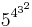
\includegraphics[scale=.9]{graphics/2869715b8204450d9946d9dd1966f50f.png}
% \caption{5\^{}\{4\^{}\{3\^{}2\}\}}
\end{figure}

\begin{itemize}
\item
  Confirm that the first and last twenty digits of the answer are: \\
  \texttt{62060698786608744707...92256259918212890625}
\item
  Find and show the number of decimal digits in the answer.
\end{itemize}

C.F. \href{/wiki/Long\_multiplication}{Long multiplication}

Note:

\begin{itemize}
\item Do not submit an \emph{implementation} of
  \href{http://en.wikipedia.org/wiki/arbitrary\_precision\_arithmetic}{arbitrary
    precision arithmetic}. The intention is to show the capabilities
  of the language as supplied. If a language has a \emph{single,
    overwhelming, library} of varied modules that is endorsed by its
  home site -- such as \emph{CPAN} for Perl or \emph{Boost} for C++ --
  then that \emph{may} be used instead.
\item
  Strictly speaking, this should not be solved by fixed-precision
  numeric libraries where the precision has to be manually set to a
  large value; although if this is the \textbf{only} recourse then it
  may be used with a note explaining that the precision must be set
  manually to a large enough value.
\end{itemize}

\begin{wideverbatim}

(let L (chop (** 5 (** 4 (** 3 2))))
   (prinl (head 20 L) "..." (tail 20 L))
   (length L) )

Output:

62060698786608744707...92256259918212890625
-> 183231

\end{wideverbatim}

\pagebreak{}
\section*{Arena storage pool}

Dynamically allocated objects take their memory from a \emph{heap}.
The memory for an object is provided by an \textbf{allocator} which
maintains the storage pool used for the \emph{heap}. Often a call to
allocator is denoted as

\begin{wideverbatim}
   P := new T
\end{wideverbatim}

where T is the type of an allocated object and P is a \emph{reference}
to the object.

The storage pool chosen by the allocator can be determined by either:

\begin{itemize}
\item
  the object type T;
\item
  the type of pointer P.
\end{itemize}

In the former case objects can be allocated only in one storage pool.
In the latter case objects of the type can be allocated in any storage
pool or on the \emph{stack}.

\textbf{Task description}\\ The task is to show how allocators and
user-defined storage pools are supported by the language. In particular:

\begin{enumerate}
\item
  define an arena storage pool. An arena is a pool in which objects are
  allocated individually, but freed by groups.
\item
  allocate some objects (e.g., integers) in the pool.
\end{enumerate}

Explain what controls the storage pool choice in the language.



\begin{wideverbatim}

PicoLisp allocates any kind of data from a single pool, because everything
is built out of a "cell" primitive. Most of this allocation happens
automatically, but can also be done explicitly with
'[http://software-lab.de/doc/refN.html#new new]' or
'[http://software-lab.de/doc/refB.html#box box]'. For memory-allocated
objects, there is no explicit way of freeing them. Database objects can be
freed with '[http://software-lab.de/doc/refZ.html#zap zap]'.

\end{wideverbatim}

\pagebreak{}
\section*{Arithmetic evaluation}


Create a program which parses and evaluates arithmetic expressions.

\begin{description}
\item[Requirements]
\end{description}

\begin{itemize}
\item
  An
  \href{http://en.wikipedia.org/wiki/Abstract\_syntax\_tree}{abstract-syntax
  tree} (AST) for the expression must be created from parsing the input.
\item
  The AST must be used in evaluation, also, so the input may not be
  directly evaluated (e.g. by calling eval or a similar language
  feature.)
\item
  The expression will be a string or list of symbols like ``(1+3)*7''.
\item
  The four symbols + - * / must be supported as binary operators with
  conventional precedence rules.
\item
   Precedence-control parentheses must also be supported.
\end{itemize}

\begin{description}
\item[Note]
\end{description}

For those who don't remember, mathematical precedence is as follows:

\begin{itemize}
\item
  Parentheses
\item
  Multiplication/Division (left to right)
\item
  Addition/Subtraction (left to right)
\end{itemize}

\begin{description}
\item[C.f]
\end{description}

\begin{itemize}
\item
  \emph{24 game Player}.
\item
  \emph{Parsing/RPN calculator algorithm}.
\item
  \emph{Parsing/RPN to infix conversion}.
\end{itemize}


\begin{wideverbatim}

The built-in function 'str' splits a string into a list of lexical tokens
(numbers and transient symbols). From that, a recursive descendent parser can
build an expression tree, resulting in directly executable Lisp code.

(de ast (Str)
   (let *L (str Str "")
      (aggregate) ) )

(de aggregate ()
   (let X (product)
      (while (member (car *L) '("+" "-"))
         (setq X (list (intern (pop '*L)) X (product))) )
      X ) )

(de product ()
   (let X (term)
      (while (member (car *L) '("*" "/"))
         (setq X (list (intern (pop '*L)) X (term))) )
      X ) )

(de term ()
   (let X (pop '*L)
      (cond
         ((num? X) X)
         ((= "+" X) (term))
         ((= "-" X) (list '- (term)))
         ((= "(" X) (prog1 (aggregate) (pop '*L)))) ) ) )

Output:

: (ast "1+2+3*-4/(1+2)")
-> (+ (+ 1 2) (/ (* 3 (- 4)) (+ 1 2)))

: (ast "(1+2+3)*-4/(1+2)")
-> (/ (* (+ (+ 1 2) 3) (- 4)) (+ 1 2))

\end{wideverbatim}

\pagebreak{}
\section*{Arithmetic-geometric mean}

Write a function to compute the
\href{http://en.wikipedia.org/wiki/Arithmetic-geometric\_mean}{arithmetic-geometric
  mean} of two numbers. The arithmetic-geometric mean of two numbers
can be (usefully) denoted as agm(\emph{a},\emph{g}), and is equal to
the limit of the sequence:

\begin{figure}[H]
\centering
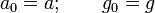
\includegraphics[scale=.6]{graphics/da869c8260ae3107ca34619fd2642642.png}
% \caption{a\_0 = a; \textbackslash{}qquad g\_0 = g}
\end{figure}

\begin{figure}[H]
\centering
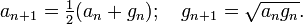
\includegraphics[scale=.6]{graphics/7416c556a1ecfe80d64f32dbc9c18ae6.png}
% \caption{a\_\{n+1\} = \textbackslash{}tfrac\{1\}\{2\}(a\_n + g\_n);
% \textbackslash{}quad g\_\{n+1\} = \textbackslash{}sqrt\{a\_n g\_n\}.}
\end{figure}

Since the limit of \emph{a}\textsubscript{\emph{n}} −
\emph{g}\textsubscript{\emph{n}} tends (rapidly) to zero with
iterations, this is an efficient method.

Demonstrate the function by calculating:

\begin{figure}[H]
\centering
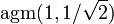
\includegraphics[scale=.6]{graphics/953f4c8f564b5ed18e1b31d2716b5f8c.png}
% \caption{\textbackslash{}mathrm\{agm\}(1,1/\textbackslash{}sqrt\{2\})}
\end{figure}



\begin{wideverbatim}

(scl 80)

(de agm (A G)
   (do 7
      (prog1 (/ (+ A G) 2)
         (setq G (sqrt (* A G))  A @) ) ) )

(round
   (agm 1.0 (*/ 1.0 1.0 (sqrt (* 2.0 1.0))))
   70 )

Output:
-> "0.8472130847939790866064991234821916364814459103269421850605793726597340"

\end{wideverbatim}

\pagebreak{}
\section*{Arithmetic/Complex}

A \textbf{\href{http://en.wikipedia.org/wiki/Complex\_number}{complex
number}} is a number which can be written as
"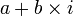
\includegraphics[scale=.6]{graphics/af18dab590e0f994693fc34b6803c1e1.png}"
(sometimes shown as
"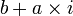
\includegraphics[scale=.6]{graphics/1465b5194836899e7331a9fcf9cda03e.png}")
where a and b are real numbers and
\href{http://en.wikipedia.org/wiki/Imaginary\_unit}{\emph{i} is the
square root of -1}. Typically, complex numbers are represented as a pair
of real numbers called the ``imaginary part'' and ``real part'', where
the imaginary part is the number to be multiplied by \emph{i}.

\begin{itemize}
\item
  Show addition, multiplication, negation, and inversion of complex
  numbers in separate functions. (Subtraction and division operations
  can be made with pairs of these operations.) Print the results for
  each operation tested.
\item
  \emph{Optional:} Show complex conjugation. By definition, the
  \href{http://en.wikipedia.org/wiki/complex\_conjugate}{complex
  conjugate} of \emph{a} + \emph{b}\emph{i} is \emph{a} −
  \emph{b}\emph{i}.
\end{itemize}

Some languages have complex number libraries available. If your language
does, show the operations. If your language does not, also show the
definition of this type.


\begin{wideverbatim}

(load "@lib/math.l")

(de addComplex (A B)
   (cons
      (+ (car A) (car B))        # Real
      (+ (cdr A) (cdr B)) ) )    # Imag

(de mulComplex (A B)
   (cons
      (-
         (*/ (car A) (car B) 1.0)
         (*/ (cdr A) (cdr B) 1.0) )
      (+
         (*/ (car A) (cdr B) 1.0)
         (*/ (cdr A) (car B) 1.0) ) ) )

(de invComplex (A)
   (let Denom
      (+
         (*/ (car A) (car A) 1.0)
         (*/ (cdr A) (cdr A) 1.0) )
      (cons
         (*/ (car A) 1.0 Denom)
         (- (*/ (cdr A) 1.0 Denom)) ) ) )

(de negComplex (A)
   (cons (- (car A)) (- (cdr A))) )

(de fmtComplex (A)
   (pack
      (round (car A) (dec *Scl))
      (and (gt0 (cdr A)) "+")
      (round (cdr A) (dec *Scl))
      "i" ) )

(let (A (1.0 . 1.0)  B (cons pi 1.2))
   (prinl "A = " (fmtComplex A))
   (prinl "B = " (fmtComplex B))
   (prinl "A+B = " (fmtComplex (addComplex A B)))
   (prinl "A*B = " (fmtComplex (mulComplex A B)))
   (prinl "1/A = " (fmtComplex (invComplex A)))
   (prinl "-A = " (fmtComplex (negComplex A))) )

Output:

A = 1.00000+1.00000i
B = 3.14159+1.20000i
A+B = 4.14159+2.20000i
A*B = 1.94159+4.34159i
1/A = 0.50000-0.50000i
-A = -1.00000-1.00000i

\end{wideverbatim}

\pagebreak{}
\section*{Arithmetic/Rational}

The objective of this task is to create a reasonably complete
implementation of rational arithmetic in the particular language using
the idioms of the language.

For example: Define a new type called \textbf{frac} with binary operator
``//'' of two integers that returns a \textbf{structure} made up of the
numerator and the denominator (as per a rational number).

Further define the appropriate rational unary \textbf{operators}
\textbf{abs} and '-', with the binary \textbf{operators} for addition
`+', subtraction '-', multiplication `×', division `/', integer division
`÷', modulo division, the comparison operators (e.g. `\textless{}', `≤',
`\textgreater{}', \& `≥') and equality operators (e.g. `=' \& `≠').

Define standard coercion \textbf{operators} for casting \textbf{int} to
\textbf{frac} etc.

If space allows, define standard increment and decrement
\textbf{operators} (e.g. `+:=' \& '-:=' etc.).

Finally test the operators: Use the new type \textbf{frac} to find all
\emph{perfect numbers} less than 2\textsuperscript{19} by summing the
reciprocal of the factors.

\textbf{See also}

\begin{itemize}
\item
  \emph{Perfect Numbers}
\end{itemize}


\begin{wideverbatim}

(load "@lib/frac.l")

(for (N 2  (> (** 2 19) N)  (inc N))
   (let (Sum (frac 1 N)  Lim (sqrt N))
      (for (F 2  (>= Lim F) (inc F))
         (when (=0 (\% N F))
            (setq Sum
               (f+ Sum
                  (f+ (frac 1 F) (frac 1 (/ N F))) ) ) ) )
      (when (= 1 (cdr Sum))
         (prinl
            "Perfect " N
            ", sum is " (car Sum)
            (and (= 1 (car Sum)) ": perfect") ) ) ) )

Output:

Perfect 6, sum is 1: perfect
Perfect 28, sum is 1: perfect
Perfect 120, sum is 2
Perfect 496, sum is 1: perfect
Perfect 672, sum is 2
Perfect 8128, sum is 1: perfect
Perfect 30240, sum is 3
Perfect 32760, sum is 3
Perfect 523776, sum is 2
\end{wideverbatim}

\pagebreak{}
\section*{Arithmetic/Integer}

\textbf{Basic Data Operation}\\ This is a basic data operation. It
represents a fundamental action on a basic data type.

You may see other such operations in the
\emph{Basic Data Operations}
category, or:

\textbf{Integer Operations} \\ \emph{Arithmetic} \textbar{}
\emph{Comparison}

\textbf{Boolean Operations} \\ \emph{Bitwise}
\textbar{} \emph{Logical}

\textbf{String Operations} \\
\emph{Concatenation} \textbar{}
\emph{Interpolation} \textbar{}
\emph{Matching}

\textbf{Memory Operations} \\
\emph{Pointers \& references}
\textbar{} \emph{Addresses}

Get two integers from the user, and then output the sum, difference,
product, integer quotient and remainder of those numbers. Don't include
error handling. For quotient, indicate how it rounds (e.g. towards 0,
towards negative infinity, etc.). For remainder, indicate whether its
sign matches the sign of the first operand or of the second operand, if
they are different.

Also include the exponentiation operator if one exists.

\begin{wideverbatim}

(de math (A B)
   (prinl "Add      " (+ A B))
   (prinl "Subtract " (- A B))
   (prinl "Multiply " (* A B))
   (prinl "Divide   " (/ A B))        # Truncates towards zero
   (prinl "Div/rnd  " (*/ A B))       # Rounds to next integer
   (prinl "Modulus  " (\% A B))        # Sign of the first operand
   (prinl "Power    " (** A B)) )

\end{wideverbatim}

\pagebreak{}
\section*{Array concatenation}

Show how to concatenate two arrays in your language. If this is as
simple as \texttt{array1 + array2}, so be it.

\begin{wideverbatim}

PicoLisp has no built-in array data type. Lists are used instead.

There are destructive concatenations:

: (setq  A (1 2 3)  B '(a b c))
-> (a b c)
: (conc A B)                        # Concatenate lists in 'A' and 'B'
-> (1 2 3 a b c)
: A
-> (1 2 3 a b c)                    # Side effect: List in 'A' is modified!

and non-destructive concatenations:

: (setq  A (1 2 3)  B '(a b c))
-> (a b c)
: (append A B)                      # Append lists in 'A' and 'B'
-> (1 2 3 a b c)
: A
-> (1 2 3)
: B
-> (a b c)                          # Arguments are not modified

\end{wideverbatim}

\pagebreak{}
\section*{Arrays}

This task is about arrays. For hashes or associative arrays, please see
\emph{Creating an Associative Array}.

In this task, the goal is to show basic array syntax in your language.
Basically, create an array, assign a value to it, and retrieve an
element. (if available, show both fixed-length arrays and dynamic
arrays, pushing a value into it.)

\textbf{See also}

\begin{itemize}
\item
  \emph{Collections}
\item
  \emph{Two-dimensional array (runtime)}
\end{itemize}


\begin{wideverbatim}

PicoLisp has no built-in array data type. Lists are used instead.

(setq A '((1 2 3) (a b c) ((d e) NIL 777)))  # Create a 3x3 structure
(mapc println A)  # Show it

Output:

(1 2 3)
(a b c)
((d e) NIL 777)

Replace 'b' with 'B' in middle row:

(set (nth A 2 2) 'B)
(mapc println A)

Output:

(1 2 3)
(a B c)
((d e) NIL 777)

Insert '1' in front of the middle row:

(push (cdr A) 1)
(mapc println A)

Output:

(1 2 3)
(1 a B c)
((d e) NIL 777)

Append '9' to the middle row:

(queue (cdr A) 9)
(mapc println A)

Output:

(1 2 3)
(1 a B c 9)
((d e) NIL 777)

\end{wideverbatim}

\pagebreak{}
\section*{Assertions}

Assertions are a way of breaking out of code when there is an error or
an unexpected input. Some languages throw \emph{exceptions} and some
treat it as a break point.

Show an assertion in your language by asserting that an integer variable
is equal to 42.

\begin{wideverbatim}

The '[http://software-lab.de/doc/refA.html#assert assert]' function, in
combination with the tilde read macro, generates code only in debug mode:

...
~(assert (= N 42))  # Exists only in debug mode
...

Other possibilities are either to break into an error handler:

(let N 41
   (unless (= N 42) (quit "Incorrect N" N)) )  # 'quit' throws an error
41 -- Incorrect N
?

or to stop at a debug break point, allowing to continue with the program:

(let N 41
   (unless (= N 42) (! setq N 42)) )   # '!' is a breakpoint
(setq N 42)                            # Manually fix the value
!                                      # Hit ENTER to leave the breakpoint
-> 42

\end{wideverbatim}

\pagebreak{}
\section*{Associative arrays/Creation}

In this task, the goal is to create an \emph{associative array} (also
known as a dictionary, map, or hash).

\begin{itemize}
\item
  Related task: \emph{Associative arrays/Iteration}
\end{itemize}


\begin{wideverbatim}

Here we use symbol properties. Other possiblities could be index
trees or association lists.

(put 'A 'foo 5)
(put 'A 'bar 10)
(put 'A 'baz 15)
(put 'A 'foo 20)

: (get 'A 'bar)
-> 10

: (get 'A 'foo)
-> 20

: (show 'A)
A NIL
   foo 20
   bar 10
   baz 15

\end{wideverbatim}

\pagebreak{}
\section*{Associative arrays/Iteration}

Show how to iterate over the key-value pairs of an associative array,
and print each pair out. Also show how to iterate just over the keys, or
the values, if there is a separate way to do that in your language.

\begin{itemize}
\item
  Related task: \emph{Associative arrays/Creation}
\end{itemize}


\begin{wideverbatim}

# Using properties

(put 'A 'foo 5)
(put 'A 'bar 10)
(put 'A 'baz 15)

: (getl 'A)                            # Get the whole property list
-> ((15 . baz) (10 . bar) (5 . foo))

: (mapcar cdr (getl 'A))               # Get all keys
-> (baz bar foo)

: (mapcar car (getl 'A))               # Get all values
-> (15 10 5)

# Using an index tree

(idx 'A (def "foo" 5) T)
(idx 'A (def "bar" 10) T)
(idx 'A (def "baz" 15) T)

: A                                    # Get the whole tree
-> ("foo" ("bar" NIL "baz"))

:  (idx 'A)                            # Get all keys
-> ("bar" "baz" "foo")

:  (mapcar val (idx 'A))               # Get all values
-> (10 15 5)

\end{wideverbatim}

\pagebreak{}
\section*{Atomic updates}

Define a data type consisting of a fixed number of `buckets', each
containing a nonnegative integer value, which supports operations to

\begin{enumerate}
\item
  get the current value of any bucket
\item
  remove a specified amount from one specified bucket and add it to
  another, preserving the total of all bucket values, and
  \href{http://en.wikipedia.org/wiki/Clamping\_(graphics)}{clamping} the
  transferred amount to ensure the values remain nonnegative
\end{enumerate}

\begin{center}\rule{3in}{0.4pt}\end{center}

In order to exercise this data type, create one set of buckets, and
start three concurrent tasks:

\begin{enumerate}
\item
  As often as possible, pick two buckets and make their values closer to
  equal.
\item
  As often as possible, pick two buckets and arbitrarily redistribute
  their values.
\item
  At whatever rate is convenient, display (by any means) the total value
  and, optionally, the individual values of each bucket.
\end{enumerate}

The display task need not be explicit; use of e.g. a debugger or trace
tool is acceptable provided it is simple to set up to provide the
display.

\begin{center}\rule{3in}{0.4pt}\end{center}

This task is intended as an exercise in \emph{atomic} operations. The
sum of the bucket values must be preserved even if the two tasks attempt
to perform transfers simultaneously, and a straightforward solution is
to ensure that at any time, only one transfer is actually occurring ---
that the transfer operation is \emph{atomic}.


\begin{wideverbatim}

(de *Buckets . 15)  # Number of buckets

# E/R model
(class +Bucket +Entity)
(rel key (+Key +Number))  # Key  1 .. *Buckets
(rel val (+Number))       # Value 1 .. 999


# Start with an empty DB
(call 'rm "-f" "buckets.db")  # Remove old DB (if any)
(pool "buckets.db")           # Create new DB file


# Create *Buckets buckets with values between 1 and 999
(for K *Buckets
   (new T '(+Bucket)  'key K  'val (rand 1 999)) )
(commit)


# Pick a random bucket
(de pickBucket ()
   (db 'key '+Bucket (rand 1 *Buckets)) )


\end{wideverbatim}

\begin{wideverbatim}

# First process
(unless (fork)
   (seed *Pid)  # Ensure local random sequence
   (loop
      (let (B1 (pickBucket)  B2 (pickBucket))  # Pick two buckets 'B1' and 'B2'
         (dbSync)                              # Atomic DB operation
         (let (V1 (; B1 val)  V2 (; B2 val))   # Get current values
            (cond
               ((> V1 V2)
                  (dec> B1 'val)               # Make them closer to equal
                  (inc> B2 'val) )
               ((> V2 V1)
                  (dec> B2 'val)
                  (inc> B1 'val) ) ) )
         (commit 'upd) ) ) )                   # Close transaction

\end{wideverbatim}

\begin{wideverbatim}

# Second process
(unless (fork)
   (seed *Pid)  # Ensure local random sequence
   (loop
      (let (B1 (pickBucket)  B2 (pickBucket))  # Pick two buckets 'B1' and 'B2'
         (unless (== B1 B2)                    # Found two different ones?
            (dbSync)                              # Atomic DB operation
            (let (V1 (; B1 val)  V2 (; B2 val))   # Get current values
               (cond
                  ((> V1 V2 0)
                     (inc> B1 'val)               # Redistribute them
                     (dec> B2 'val) )
                  ((> V2 V1 0)
                     (inc> B2 'val)
                     (dec> B1 'val) ) ) )
            (commit 'upd) ) ) ) )                 # Close transaction


\end{wideverbatim}

\begin{wideverbatim}

# Third process
(unless (fork)
   (loop
      (dbSync)                         # Atomic DB operation
      (let Lst (collect 'key '+Bucket) # Get all buckets
         (for This Lst                 # Print current values
            (printsp (: val)) )
         (prinl                        # and total sum
            "-- Total: "
            (sum '((This) (: val)) Lst) ) )
      (rollback)
      (wait 2000) ) )                  # Sleep two seconds

(wait)

\end{wideverbatim}

\begin{wideverbatim}

Output:

70 236 582 30 395 215 525 653 502 825 129 769 722 440 708 -- Total: 6801
0 156 566 352 198 263 0 743 0 1316 58 1180 897 0 1072 -- Total: 6801
0 0 424 101 0 0 0 682 0 1809 0 1549 961 0 1275 -- Total: 6801
0 0 0 0 0 0 0 452 0 2226 0 1838 884 0 1401 -- Total: 6801
54 55 56 55 54 55 54 102 54 2363 54 1816 666 55 1308 -- Total: 6801
198 198 197 196 198 198 197 197 196 1903 197 1438 345 197 946 -- Total: 6801
342 344 343 344 344 342 344 343 343 1278 343 992 343 343 413 -- Total: 6801
^C

\end{wideverbatim}

\pagebreak{}
\section*{Averages/Arithmetic mean}

Write a program to find the
\href{http://en.wikipedia.org/wiki/arithmetic\_mean}{mean} (arithmetic
average) of a numeric vector. In case of a zero-length input, since
the mean of an empty set of numbers is ill-defined, the program may
choose to behave in any way it deems appropriate, though if the
programming language has an established convention for conveying math
errors or undefined values, it's preferable to follow it.

See also: \emph{Median}, \emph{Mode}

\begin{wideverbatim}

(de mean (Lst)
   (if (atom Lst)
      0
      (/ (apply + Lst) (length Lst)) ) )

Output:

: (mean (range 1 1000))
-> 500

\end{wideverbatim}


\pagebreak{}
\section*{Averages/Mean angle}

When calculating the
\href{http://en.wikipedia.org/wiki/Mean\_of\_circular\_quantities}{average
  or mean of an angle} one has to take into account how angles wrap
around so that any angle in degrees plus any integer multiple of 360
degrees is a measure of the same angle.

If one wanted an average direction of the wind over two readings where
the first reading was of 350 degrees and the second was of 10 degrees
then just using the Pythagorean average of the numbers yields an answer
of 180 degrees, whereas if you can note that 350 degrees is equivalent
to -10 degrees and so you have two readings at 10 degrees either side of
zero degrees leading to a more fitting mean angle of zero degrees.

To calculate the mean angle of several angles:

\begin{enumerate}
\item
  Assume all angles are on the unit circle and convert them to complex
  numbers expressed in real and imaginary form.
\item
  Compute the Pythagorean mean of the complex numbers.
\item
  Convert the complex mean to polar coordinates whereupon the phase of
  the complex mean is the required angular mean.
\end{enumerate}

(Note that, since the mean is the sum divided by the number of numbers,
and division by a positive real number does not affect the angle, you
can also simply compute the sum for step 2.)

You can alternatively use this formula:

Given the
angles 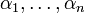
\includegraphics[scale=.6]{graphics/e5d832c5ee9a16553e635e05c2892174.png}
the mean is computed by

\begin{figure}[H]
\centering
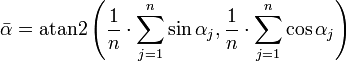
\includegraphics[scale=.6]{graphics/1a4bfb06a8eb34d1ac09405c02d064c4.png}
% \caption{\textbackslash{}bar\{\textbackslash{}alpha\} =
% \textbackslash{}operatorname\{atan2\}\textbackslash{}left(\textbackslash{}frac\{1\}\{n\}\textbackslash{}cdot\textbackslash{}sum\_\{j=1\}\^{}n
% \textbackslash{}sin\textbackslash{}alpha\_j,
% \textbackslash{}frac\{1\}\{n\}\textbackslash{}cdot\textbackslash{}sum\_\{j=1\}\^{}n
% \textbackslash{}cos\textbackslash{}alpha\_j\textbackslash{}right) }
\end{figure}

The task is to:

\begin{enumerate}
\item
  write a function/method/subroutine/\ldots{} that given a list of
  angles in degrees returns their mean angle. (You should use a built-in
  function if you have one that does this for degrees or radians).
\item
  Use the function to compute the means of these lists of angles (in
  degrees): {[}350, 10{]}, {[}90, 180, 270, 360{]}, {[}10, 20, 30{]};
  and show your output here.
\end{enumerate}


\begin{wideverbatim}

(load "@lib/math.l")
 
(de meanAngle (Lst)
   (*/
      (atan2
         (sum '((A) (sin (*/ A pi 180.0))) Lst)
         (sum '((A) (cos (*/ A pi 180.0))) Lst) )
      180.0 pi ) )
 
(for L '((350.0 10.0) (90.0 180.0 270.0 360.0) (10.0 20.0 30.0))
   (prinl
      "The mean angle of ["
      (glue ", " (mapcar round L '(0 .)))
      "] is: " (round (meanAngle L))) )

Output:

The mean angle of [350, 10] is: 0.000
The mean angle of [90, 180, 270, 360] is: 90.000
The mean angle of [10, 20, 30] is: 20.000

\end{wideverbatim}


\pagebreak{}
\section*{Averages/Mean time of day}

A particular activity of bats occurs at these times of the day:

\texttt{23:00:17, 23:40:20, 00:12:45, 00:17:19}

Using the idea that their are twenty four hours in a day which is
analogous to their being 360 degrees in a circle, map times of day to
and from angles and using the ideas of \emph{Averages/Mean angle}
compute and show here the average time of the nocturnal activity to an
accuracy of a second of time.


\begin{wideverbatim}

(load "@lib/math.l")
 
(de meanTime (Lst)
   (let Tim
      (*/
         (atan2
            (sum '((S) (sin (*/ ($tim S) pi 43200))) Lst)
            (sum '((S) (cos (*/ ($tim S) pi 43200))) Lst) )
         43200 pi )
      (tim$ (% (+ Tim 86400) 86400) T) ) )

Test:

: (meanTime '("23:00:17" "23:40:20" "00:12:45" "00:17:19"))
-> "23:47:43"

\end{wideverbatim}

\pagebreak{}
\section*{Averages/Median}

Write a program to find the
\href{http://en.wikipedia.org/wiki/Median}{median} value of a vector
of floating-point numbers. The program need not handle the case where
the vector is empty, but \emph{must} handle the case where there are
an even number of elements.

There are several approaches to this. One is to sort the elements, and
then pick the one in the middle. Sorting would take at least
O(\emph{n}log\emph{n}). Another would be to build a priority queue
from the elements, and then extract half of the elements to get to the
middle one(s). This would also take O(\emph{n}log\emph{n}). The best
solution is to use the
\href{http://en.wikipedia.org/wiki/Selection\_algorithm}{selection
  algorithm} to find the median in O(\emph{n}) time.

See also: \emph{Mean}, \emph{Mode}

\begin{wideverbatim}

(de median (Lst)
   (let N (length Lst)
      (if (bit? 1 N)
         (get (sort Lst) (/ (inc N) 2))
         (setq Lst (nth (sort Lst) (/ N 2)))
         (/ (+ (car Lst) (cadr Lst)) 2) ) ) )

(scl 2)
(prinl (round (median (1.0 2.0 3.0))))
(prinl (round (median (1.0 2.0 3.0 4.0))))
(prinl (round (median (5.1 2.6 6.2 8.8 4.6 4.1))))
(prinl (round (median (5.1 2.6 8.8 4.6 4.1))))

Output:

2.00
2.50
4.85
4.60

\end{wideverbatim}

\pagebreak{}
\section*{Averages/Mode}

Write a program to find the
\href{http://en.wikipedia.org/wiki/Mode\_(statistics)}{mode} value of
a collection. The case where the collection is empty may be ignored.
Care must be taken to handle the case where the mode is non-unique.

If it is not appropriate or possible to support a general collection,
use a vector (array), if possible. If it is not appropriate or possible
to support an unspecified value type, use integers.

See also: \emph{Mean},\emph{Median}

\begin{wideverbatim}

(de modes (Lst)
   (let A NIL
      (for X Lst
         (accu 'A X 1) )
      (mapcar car
         (maxi cdar
            (by cdr group A) ) ) ) )

Output:

: (modes (1 3 6 6 6 6 7 7 12 12 17))
-> (6)

: (modes (1 1 2 4 4))
-> (4 1)

: (modes (chop "ABRAHAMASANTACLARA"))
-> ("A")

: (modes (1 4 A 3 2 7 1 B B 3 6 2 4 C C 5 2 5 B A 3 2 C 3 5 5 4 C 7 7))
-> (5 C 2 3)

\end{wideverbatim}

\pagebreak{}
\section*{Averages/Pythagorean means}


Compute all three of the
\href{http://en.wikipedia.org/wiki/Pythagorean\_means}{Pythagorean
means} of the set of integers 1 through 10.

Show that \\
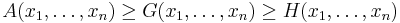
\includegraphics[scale=.6]{graphics/6d547901f0a5fb3819d16aca0048b3ed.png} \\
for this set of positive integers.

\begin{itemize}
\item The most common of the three means, the \emph{arithmetic mean},
  is the sum of the list divided by its length:
\end{itemize}

\begin{figure}[H]
\centering
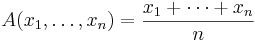
\includegraphics[scale=.6]{graphics/2b72903b5dd461c777da13fde57f3ebb.png}
% \caption{ A(x\_1, \textbackslash{}ldots, x\_n) =
% \textbackslash{}frac\{x\_1 + \textbackslash{}cdots + x\_n\}\{n\}}
\end{figure}

\begin{itemize}
\item
  The \href{http://en.wikipedia.org/wiki/Geometric\_mean}{geometric
  mean} is the \emph{n}th root of the product of the list:
\end{itemize}

\begin{figure}[H]
\centering
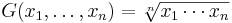
\includegraphics[scale=.6]{graphics/12595bb2b15b5d8b7263aba68c137db3.png}
% \caption{ G(x\_1, \textbackslash{}ldots, x\_n) =
% \textbackslash{}sqrt{[}n{]}\{x\_1 \textbackslash{}cdots x\_n\} }
\end{figure}

\begin{itemize}
\item
  The \href{http://en.wikipedia.org/wiki/Harmonic\_mean}{harmonic mean}
  is \emph{n} divided by the sum of the reciprocal of each item in the
  list:
\end{itemize}

\begin{figure}[H]
\centering
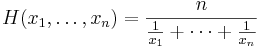
\includegraphics[scale=.6]{graphics/7f1c92a1977747914e9c5127764a9be4.png}
% \caption{ H(x\_1, \textbackslash{}ldots, x\_n) =
% \textbackslash{}frac\{n\}\{\textbackslash{}frac\{1\}\{x\_1\} +
% \textbackslash{}cdots + \textbackslash{}frac\{1\}\{x\_n\}\} }
\end{figure}

C.f. \emph{Averages/Root mean square}


\begin{wideverbatim}

(load "@lib/math.l")

(let (Lst (1.0 2.0 3.0 4.0 5.0 6.0 7.0 8.0 9.0 10.0)  Len (length Lst))
   (prinl "Arithmetic mean: "
      (format
         (/ (apply + Lst) Len)
         *Scl ) )
   (prinl "Geometric mean: "
      (format
         (pow (*/ (apply * Lst) (** 1.0 (dec Len))) (/ 1.0 Len))
         *Scl ) )
   (prinl "Harmonic mean: "
      (format
         (*/ (* 1.0 Len) 1.0 (sum '((N) (*/ 1.0 1.0 N)) Lst))
         *Scl ) ) )

Output:

Arithmetic mean: 5.500000
Geometric mean: 4.528729
Harmonic mean: 3.414172

\end{wideverbatim}

\pagebreak{}
\section*{Averages/Root mean square}

Compute the \href{http://en.wikipedia.org/wiki/Root\_mean\_square}{Root
mean square} of the numbers 1..10.

The root mean square is also known by its initial RMS (or rms), and as
the \textbf{quadratic mean}.

The RMS is calculated as the mean of the squares of the numbers,
square-rooted:

\begin{figure}[H]
\centering
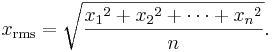
\includegraphics[scale=.6]{graphics/cf22c76e0c33c4fb96262638a28bd52b.png}
% \caption{x\_\{\textbackslash{}mathrm\{rms\}\} = \textbackslash{}sqrt
% \{\{\{x\_1\}\^{}2 + \{x\_2\}\^{}2 + \textbackslash{}cdots +
% \{x\_n\}\^{}2\} \textbackslash{}over n\}. }
\end{figure}

Cf. \emph{Averages/Pythagorean means}


\begin{wideverbatim}

(scl 5)

(let Lst (1.0 2.0 3.0 4.0 5.0 6.0 7.0 8.0 9.0 10.0)
   (prinl
      (format
         (sqrt
            (*/
               (sum '((N) (*/ N N 1.0)) Lst)
               1.0
               (length Lst) )
            T )
         *Scl ) ) )

Output:

6.20484

\end{wideverbatim}

\pagebreak{}
\section*{Averages/Simple moving average}


Computing the
\href{http://en.wikipedia.org/wiki/Moving\_average\#Simple\_moving\_average}{simple
moving average} of a series of numbers.

The task is to:

\emph{Create a \href{http://en.wikipedia.org/wiki/Stateful}{stateful}
function/class/instance that takes a period and returns a routine that
takes a number as argument and returns a simple moving average of its
arguments so far.}

\textbf{Description}\\ A simple moving average is a method for computing
an average of a stream of numbers by only averaging the last P numbers
from the stream, where P is known as the period. It can be implemented
by calling an initialing routine with P as its argument, I(P), which
should then return a routine that when called with individual,
successive members of a stream of numbers, computes the mean of (up to),
the last P of them, lets call this SMA().

The word stateful in the task description refers to the need for SMA()
to remember certain information between calls to it:

\begin{itemize}
\item
  The period, P
\item
  An ordered container of at least the last P numbers from each of its
  individual calls.
\end{itemize}

Stateful also means that successive calls to I(), the initializer,
should return separate routines that do \emph{not} share saved state so
they could be used on two independent streams of data.

Pseudocode for an implementation of SMA is:

\begin{wideverbatim}
function SMA(number: N):
    stateful integer: P
    stateful list:    stream
    number:           average

    stream.append_last(N)
    if stream.length() > P:
        # Only average the last P elements of the stream
        stream.delete_first()
    if stream.length() == 0:
        average = 0
    else:    
        average = sum( stream.values() ) / stream.length()
    return average
\end{wideverbatim}

 See also: \emph{Standard Deviation}


\begin{wideverbatim}

(de sma (@Len)
   (curry (@Len (Data)) (N)
      (push 'Data N)
      (and (nth Data @Len) (con @))  # Truncate
      (*/ (apply + Data) (length Data)) ) )


(def 'sma3 (sma 3))
(def 'sma5 (sma 5))

(scl 2)
(for N (1.0 2.0 3.0 4.0 5.0 5.0 4.0 3.0 2.0 1.0)
   (prinl
      (format N *Scl)
      "   (sma3) "
      (format (sma3 N) *Scl)
      "   (sma5) "
      (format (sma5 N) *Scl) ) )

Output:

1.00   (sma3) 1.00   (sma5) 1.00
2.00   (sma3) 1.50   (sma5) 1.50
3.00   (sma3) 2.00   (sma5) 2.00
4.00   (sma3) 3.00   (sma5) 2.50
5.00   (sma3) 4.00   (sma5) 3.00
5.00   (sma3) 4.67   (sma5) 3.80
4.00   (sma3) 4.67   (sma5) 4.20
3.00   (sma3) 4.00   (sma5) 4.20
2.00   (sma3) 3.00   (sma5) 3.80
1.00   (sma3) 2.00   (sma5) 3.00

\end{wideverbatim}


% %%%%%%%%%%%%%%%%%%%%%%%% referenc.tex %%%%%%%%%%%%%%%%%%%%%%%%%%%%%%
% sample references
% %
% Use this file as a template for your own input.
%
%%%%%%%%%%%%%%%%%%%%%%%% Springer-Verlag %%%%%%%%%%%%%%%%%%%%%%%%%%
%
% BibTeX users please use
% \bibliographystyle{}
% \bibliography{}
%
\biblstarthook{In view of the parallel print and (chapter-wise) online publication of your book at \url{www.springerlink.com} it has been decided that -- as a genreral rule --  references should be sorted chapter-wise and placed at the end of the individual chapters. However, upon agreement with your contact at Springer you may list your references in a single seperate chapter at the end of your book. Deactivate the class option \texttt{sectrefs} and the \texttt{thebibliography} environment will be put out as a chapter of its own.\\\indent
References may be \textit{cited} in the text either by number (preferred) or by author/year.\footnote{Make sure that all references from the list are cited in the text. Those not cited should be moved to a separate \textit{Further Reading} section or chapter.} The reference list should ideally be \textit{sorted} in alphabetical order -- even if reference numbers are used for the their citation in the text. If there are several works by the same author, the following order should be used: 
\begin{enumerate}
\item all works by the author alone, ordered chronologically by year of publication
\item all works by the author with a coauthor, ordered alphabetically by coauthor
\item all works by the author with several coauthors, ordered chronologically by year of publication.
\end{enumerate}
The \textit{styling} of references\footnote{Always use the standard abbreviation of a journal's name according to the ISSN \textit{List of Title Word Abbreviations}, see \url{http://www.issn.org/en/node/344}} depends on the subject of your book:
\begin{itemize}
\item The \textit{two} recommended styles for references in books on \textit{mathematical, physical, statistical and computer sciences} are depicted in ~\cite{science-contrib, science-online, science-mono, science-journal, science-DOI} and ~\cite{phys-online, phys-mono, phys-journal, phys-DOI, phys-contrib}.
\item Examples of the most commonly used reference style in books on \textit{Psychology, Social Sciences} are~\cite{psysoc-mono, psysoc-online,psysoc-journal, psysoc-contrib, psysoc-DOI}.
\item Examples for references in books on \textit{Humanities, Linguistics, Philosophy} are~\cite{humlinphil-journal, humlinphil-contrib, humlinphil-mono, humlinphil-online, humlinphil-DOI}.
\item Examples of the basic Springer style used in publications on a wide range of subjects such as \textit{Computer Science, Economics, Engineering, Geosciences, Life Sciences, Medicine, Biomedicine} are ~\cite{basic-contrib, basic-online, basic-journal, basic-DOI, basic-mono}. 
\end{itemize}
}

\begin{thebibliography}{99.}%
% and use \bibitem to create references.
%
% Use the following syntax and markup for your references if 
% the subject of your book is from the field 
% "Mathematics, Physics, Statistics, Computer Science"
%
% Contribution 
\bibitem{science-contrib} Broy, M.: Software engineering --- from auxiliary to key technologies. In: Broy, M., Dener, E. (eds.) Software Pioneers, pp. 10-13. Springer, Heidelberg (2002)
%
% Online Document
\bibitem{science-online} Dod, J.: Effective substances. In: The Dictionary of Substances and Their Effects. Royal Society of Chemistry (1999) Available via DIALOG. \\
\url{http://www.rsc.org/dose/title of subordinate document. Cited 15 Jan 1999}
%
% Monograph
\bibitem{science-mono} Geddes, K.O., Czapor, S.R., Labahn, G.: Algorithms for Computer Algebra. Kluwer, Boston (1992) 
%
% Journal article
\bibitem{science-journal} Hamburger, C.: Quasimonotonicity, regularity and duality for nonlinear systems of partial differential equations. Ann. Mat. Pura. Appl. \textbf{169}, 321--354 (1995)
%
% Journal article by DOI
\bibitem{science-DOI} Slifka, M.K., Whitton, J.L.: Clinical implications of dysregulated cytokine production. J. Mol. Med. (2000) doi: 10.1007/s001090000086 
%
\bigskip

% Use the following (APS) syntax and markup for your references if 
% the subject of your book is from the field 
% "Mathematics, Physics, Statistics, Computer Science"
%
% Online Document
\bibitem{phys-online} J. Dod, in \textit{The Dictionary of Substances and Their Effects}, Royal Society of Chemistry. (Available via DIALOG, 1999), 
\url{http://www.rsc.org/dose/title of subordinate document. Cited 15 Jan 1999}
%
% Monograph
\bibitem{phys-mono} H. Ibach, H. L\"uth, \textit{Solid-State Physics}, 2nd edn. (Springer, New York, 1996), pp. 45-56 
%
% Journal article
\bibitem{phys-journal} S. Preuss, A. Demchuk Jr., M. Stuke, Appl. Phys. A \textbf{61}
%
% Journal article by DOI
\bibitem{phys-DOI} M.K. Slifka, J.L. Whitton, J. Mol. Med., doi: 10.1007/s001090000086
%
% Contribution 
\bibitem{phys-contrib} S.E. Smith, in \textit{Neuromuscular Junction}, ed. by E. Zaimis. Handbook of Experimental Pharmacology, vol 42 (Springer, Heidelberg, 1976), p. 593
%
\bigskip
%
% Use the following syntax and markup for your references if 
% the subject of your book is from the field 
% "Psychology, Social Sciences"
%
%
% Monograph
\bibitem{psysoc-mono} Calfee, R.~C., \& Valencia, R.~R. (1991). \textit{APA guide to preparing manuscripts for journal publication.} Washington, DC: American Psychological Association.
%
% Online Document
\bibitem{psysoc-online} Dod, J. (1999). Effective substances. In: The dictionary of substances and their effects. Royal Society of Chemistry. Available via DIALOG. \\
\url{http://www.rsc.org/dose/Effective substances.} Cited 15 Jan 1999.
%
% Journal article
\bibitem{psysoc-journal} Harris, M., Karper, E., Stacks, G., Hoffman, D., DeNiro, R., Cruz, P., et al. (2001). Writing labs and the Hollywood connection. \textit{J Film} Writing, 44(3), 213--245.
%
% Contribution 
\bibitem{psysoc-contrib} O'Neil, J.~M., \& Egan, J. (1992). Men's and women's gender role journeys: Metaphor for healing, transition, and transformation. In B.~R. Wainrig (Ed.), \textit{Gender issues across the life cycle} (pp. 107--123). New York: Springer.
%
% Journal article by DOI
\bibitem{psysoc-DOI}Kreger, M., Brindis, C.D., Manuel, D.M., Sassoubre, L. (2007). Lessons learned in systems change initiatives: benchmarks and indicators. \textit{American Journal of Community Psychology}, doi: 10.1007/s10464-007-9108-14.
%
%
% Use the following syntax and markup for your references if 
% the subject of your book is from the field 
% "Humanities, Linguistics, Philosophy"
%
\bigskip
%
% Journal article
\bibitem{humlinphil-journal} Alber John, Daniel C. O'Connell, and Sabine Kowal. 2002. Personal perspective in TV interviews. \textit{Pragmatics} 12:257--271
%
% Contribution 
\bibitem{humlinphil-contrib} Cameron, Deborah. 1997. Theoretical debates in feminist linguistics: Questions of sex and gender. In \textit{Gender and discourse}, ed. Ruth Wodak, 99--119. London: Sage Publications.
%
% Monograph
\bibitem{humlinphil-mono} Cameron, Deborah. 1985. \textit{Feminism and linguistic theory.} New York: St. Martin's Press.
%
% Online Document
\bibitem{humlinphil-online} Dod, Jake. 1999. Effective substances. In: The dictionary of substances and their effects. Royal Society of Chemistry. Available via DIALOG. \\
http://www.rsc.org/dose/title of subordinate document. Cited 15 Jan 1999
%
% Journal article by DOI
\bibitem{humlinphil-DOI} Suleiman, Camelia, Daniel C. O�Connell, and Sabine Kowal. 2002. `If you and I, if we, in this later day, lose that sacred fire...�': Perspective in political interviews. \textit{Journal of Psycholinguistic Research}. doi: 10.1023/A:1015592129296.
%
%
%
\bigskip
%
%
% Use the following syntax and markup for your references if 
% the subject of your book is from the field 
% "Computer Science, Economics, Engineering, Geosciences, Life Sciences"
%
%
% Contribution 
\bibitem{basic-contrib} Brown B, Aaron M (2001) The politics of nature. In: Smith J (ed) The rise of modern genomics, 3rd edn. Wiley, New York 
%
% Online Document
\bibitem{basic-online} Dod J (1999) Effective Substances. In: The dictionary of substances and their effects. Royal Society of Chemistry. Available via DIALOG. \\
\url{http://www.rsc.org/dose/title of subordinate document. Cited 15 Jan 1999}
%
% Journal article by DOI
\bibitem{basic-DOI} Slifka MK, Whitton JL (2000) Clinical implications of dysregulated cytokine production. J Mol Med, doi: 10.1007/s001090000086
%
% Journal article
\bibitem{basic-journal} Smith J, Jones M Jr, Houghton L et al (1999) Future of health insurance. N Engl J Med 965:325--329
%
% Monograph
\bibitem{basic-mono} South J, Blass B (2001) The future of modern genomics. Blackwell, London 
%
\end{thebibliography}

